\documentclass[aspectratio=169]{beamer}

\usetheme{default}
\usepackage[T1]{fontenc}
\usepackage[utf8]{inputenc}
\usepackage{lmodern}
\usepackage{mathtools}
\usepackage{amssymb}
\usepackage{pifont}
\usepackage{tikz}
\usetikzlibrary{arrows.meta,positioning}
\usepackage{booktabs}
\usepackage{xcolor}

\definecolor{inkblue}{HTML}{1B2A4A}
\definecolor{accentgold}{HTML}{C8963E}
\definecolor{signalred}{HTML}{B33F32}
\definecolor{softgray}{HTML}{6B7280}

\setbeamercolor{title}{fg=inkblue}
\setbeamercolor{frametitle}{fg=white,bg=inkblue}
\setbeamercolor{structure}{fg=inkblue}
\setbeamercolor{block title}{fg=white,bg=inkblue}
\setbeamercolor{block body}{fg=black,bg=inkblue!6}
\setbeamertemplate{navigation symbols}{}
\setbeamertemplate{footline}[page number]

\newcommand{\as}{\xrightarrow{\text{a.s.}}}
\newcommand{\inprob}{\xrightarrow{\ P\ }}
\newcommand{\inlaw}{\xrightarrow{\ d\ }}
\newcommand{\inLp}{\xrightarrow{\ L^p\ }}
\newcommand{\ceref}[1]{\textcolor{signalred}{(CE~#1)}}

\title[Modes of Convergence]{Modes of Convergence}
\subtitle{Almost sure, in probability, $L^p$, and in law --- how they imply each other}
\date{\today}

\begin{document}

\begin{frame}
  \titlepage
\end{frame}

\begin{frame}{Outline}
  \tableofcontents
\end{frame}

\section{Definitions}

\begin{frame}{Four notions of ``$X_n \to X$''}
  Let $X_1, X_2, \dots$ and $X$ be random variables on the same probability space $(\Omega, \mathcal F, P)$.

  \vspace{2mm}
  \begin{block}{Almost surely (a.s.)}
    $X_n \as X \iff P\Big(\lim\limits_{n\to\infty} X_n = X\Big) = 1$
  \end{block}
  \begin{block}{In probability}
    $X_n \inprob X \iff \forall \varepsilon>0,\ \ P(|X_n - X| > \varepsilon) \to 0$
  \end{block}
  \begin{block}{In $L^p$, $p \ge 1$ (\textit{$p$-th mean})}
    $X_n \inLp X \iff \mathbb E\,|X_n - X|^p \to 0$
  \end{block}
  \begin{block}{In law (weakly)}
    $X_n \inlaw X \iff \mathbb E[f(X_n)] \to \mathbb E[f(X)] \ \ \forall f$ bounded continuous
  \end{block}
\end{frame}

\section{The implication map}

\begin{frame}{Which convergence implies which}
  \begin{center}
  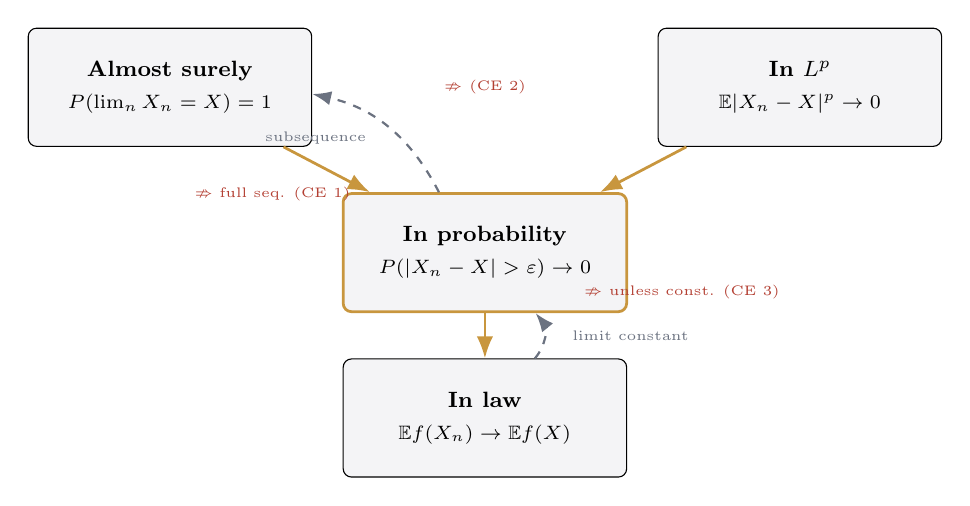
\begin{tikzpicture}[
      box/.style={draw, rounded corners=3pt, minimum width=3.6cm, minimum height=1.5cm,
                  align=center, font=\footnotesize, fill=inkblue!5},
      hub/.style={box, draw=accentgold, line width=1pt},
      arr/.style={-{Latex[length=2.8mm]}, line width=1pt, draw=accentgold},
      darr/.style={-{Latex[length=2.4mm]}, line width=0.8pt, draw=softgray,
                   dash pattern=on 3pt off 3pt}
    ]
    \node[box] (as)  at (0,3.5)  {\textbf{Almost surely}\\[2pt]\scriptsize $P(\lim_n X_n = X)=1$};
    \node[box] (lp)  at (8,3.5)  {\textbf{In $L^p$}\\[2pt]\scriptsize $\mathbb E|X_n-X|^p\to 0$};
    \node[hub] (pr)  at (4,1.4)  {\textbf{In probability}\\[2pt]\scriptsize $P(|X_n-X|>\varepsilon)\to 0$};
    \node[box] (law) at (4,-0.7) {\textbf{In law}\\[2pt]\scriptsize $\mathbb E f(X_n)\to \mathbb E f(X)$};

    \draw[arr] (as) -- (pr);
    \draw[arr] (lp) -- (pr);
    \draw[arr] (pr) -- (law);
    \draw[darr] (pr) to[bend right=25] (as);
    \draw[darr] (law) to[bend right=40] (pr);

    \node[font=\tiny, text=softgray] at (1.85,2.85) {subsequence};
    \node[font=\tiny, text=softgray] at (5.85,0.35) {limit constant};

    \node[font=\tiny, text=signalred] at (4,3.5)    {$\nRightarrow$ \ceref{2}};
    \node[font=\tiny, text=signalred] at (1.3,2.15) {$\nRightarrow$ full seq. \ceref{1}};
    \node[font=\tiny, text=signalred] at (6.5,0.9)  {$\nRightarrow$ unless const. \ceref{3}};
  \end{tikzpicture}
  \end{center}

  \vspace{1mm}
  {\scriptsize
    \textcolor{accentgold}{\textbf{---}}\ always true \qquad
    \textcolor{softgray}{\textbf{- - -}}\ true under an extra condition \qquad
    \textcolor{signalred}{$\nRightarrow$}\ false in general (see counterexample)
  }

  \vspace{2mm}
  {\scriptsize Not drawn, since it follows transitively: $L^p \Rightarrow$ in law.
  Also false in general: in probability $\nRightarrow L^1$ \ceref{4}.}
\end{frame}

\section{Counterexamples}

\begin{frame}{Counterexample 1: in probability $\nRightarrow$ almost surely}
  \textbf{Setup.} On $(\Omega,P) = ([0,1], \text{Lebesgue})$. Write each $n\ge 1$ uniquely as
  $n = 2^k + j$ with $0 \le j < 2^k$, and set
  \[ A_n = \Big[\tfrac{j}{2^k},\, \tfrac{j+1}{2^k}\Big], \qquad X_n = \mathbf 1_{A_n}. \]

  \textbf{In probability.} $P(A_n) = 2^{-k} \to 0$, so $X_n \inprob 0$.

  \textbf{Not a.s.} The intervals sweep across $[0,1]$ forever: every $\omega$ lies in
  infinitely many $A_n$ \emph{and} infinitely many complements, so $X_n(\omega)$ keeps
  oscillating between $0$ and $1$ --- it converges at no point at all.

  \vfill
  {\small\itshape the typewriter sequence}
\end{frame}

\begin{frame}{Counterexample 2: almost sure $\nRightarrow L^p$}
  \textbf{Setup.} On $([0,1], \text{Lebesgue})$, let $X_n = n \cdot \mathbf 1_{(0,\, 1/n)}$.

  \textbf{Almost surely.} For every fixed $\omega>0$, eventually $1/n < \omega$, so
  $X_n(\omega)=0$. Hence $X_n \as 0$ (and therefore also $X_n \inprob 0$).

  \textbf{Not in $L^p$.} $\mathbb E[X_n] = n \cdot \tfrac1n = 1$ for every $n$ --- the mean
  never moves. So $X_n \not\inLp 0$, for any $p \ge 1$.

  \vfill
  {\small\itshape the escaping spike --- no domination, no uniform integrability}
\end{frame}

\begin{frame}{Counterexample 3: in law $\nRightarrow$ in probability}
  \textbf{Setup.} Let $X \sim N(0,1)$ and $X_n = (-1)^n X$.

  \textbf{In law.} Since $-X \sim N(0,1)$ too, every $X_n$ has exactly the law of $X$.
  So trivially $X_n \inlaw X$.

  \textbf{Not in probability.} For odd $n$, $|X_n - X| = 2|X|$, which is not small.
  $P(|X_n-X|>\varepsilon)$ does not tend to $0$: convergence in law only pins down
  marginal distributions, never the coupling between $X_n$ and $X$.

  \vfill
  {\small\itshape same law, different variable}
\end{frame}

\begin{frame}{Counterexample 4: in probability $\nRightarrow L^1$}
  \textbf{Setup.} Reuse the typewriter sets $A_n = \big[\tfrac{j}{2^k},\tfrac{j+1}{2^k}\big]$
  from CE~1 ($n=2^k+j$), but raise the spike height with the level:
  \[ X_n = 4^k \cdot \mathbf 1_{A_n}. \]

  \textbf{In probability.} As before, $P(A_n) = 2^{-k} \to 0$, so $X_n \inprob 0$.

  \textbf{Not in $L^1$.} $\mathbb E[X_n] = 4^k \cdot 2^{-k} = 2^k \to \infty$: the mean
  doesn't just fail to vanish, it diverges. Convergence in probability puts no control
  at all on $L^1$ behaviour --- only on how \emph{often} a deviation happens, never on
  its \emph{size}.

  \vfill
  {\small\itshape the typewriter sequence, with the volume turned up}
\end{frame}

\section{Special cases}

\begin{frame}{Three repairs that restore a missing arrow}
  \begin{block}{Subsequence rescue (F.\ Riesz)}
    $X_n \inprob X \ \Rightarrow\ \exists$ a subsequence $X_{n_k} \as X$.
  \end{block}
  \begin{block}{Constant-limit rescue}
    $X_n \inlaw c$, $c$ constant $\ \Rightarrow\ X_n \inprob c$.
  \end{block}
  \begin{block}{Uniform-integrability rescue}
    $X_n \as X$ (or $\inprob$) and $\{|X_n|^p\}$ uniformly integrable
    $\ \Rightarrow\ X_n \inLp X$ (dominated convergence).
  \end{block}
\end{frame}

\section{Summary}

\begin{frame}{Every pairwise relation, at a glance}
  \centering
  \renewcommand{\arraystretch}{1.35}
  \begin{tabular}{lcccc}
    \toprule
     \textbf{if $X_n\to X$ in\ldots} & a.s. & in $P$ & $L^p$ & in law \\
    \midrule
    a.s.   & -- & \ding{51} & \textcolor{signalred}{$\nRightarrow^\ddagger$} & \ding{51} \\
    in $P$ & \textcolor{signalred}{$\nRightarrow^{*}$} & -- & \textcolor{signalred}{$\nRightarrow^\ddagger$} & \ding{51} \\
    $L^p$  & \textcolor{signalred}{$\nRightarrow^{*}$} & \ding{51} & -- & \ding{51} \\
    in law & \textcolor{signalred}{$\nRightarrow$} & \textcolor{signalred}{$\nRightarrow^\dagger$} & \textcolor{signalred}{$\nRightarrow$} & -- \\
    \bottomrule
  \end{tabular}

  \vspace{4mm}
  {\scriptsize
  $^{*}$ holds for a subsequence only (F. Riesz)\\[1pt]
  $^{\dagger}$ holds if the limit is almost-surely constant\\[1pt]
  $^{\ddagger}$ holds under an added uniform-integrability / domination condition
  }
\end{frame}

\begin{frame}{Takeaway}
  \Large
  \textit{Almost-sure and $L^p$ convergence are the strong notions; both flow through
  convergence in probability into the weakest one, convergence in law --- and none of
  the arrows run backward without borrowing an extra condition.}
\end{frame}

\end{document}
